\section{Recurrent Multi-Object Tracking with Self-Attention}
\label{sec:method}

\begin{figure}[t]
	\centering
	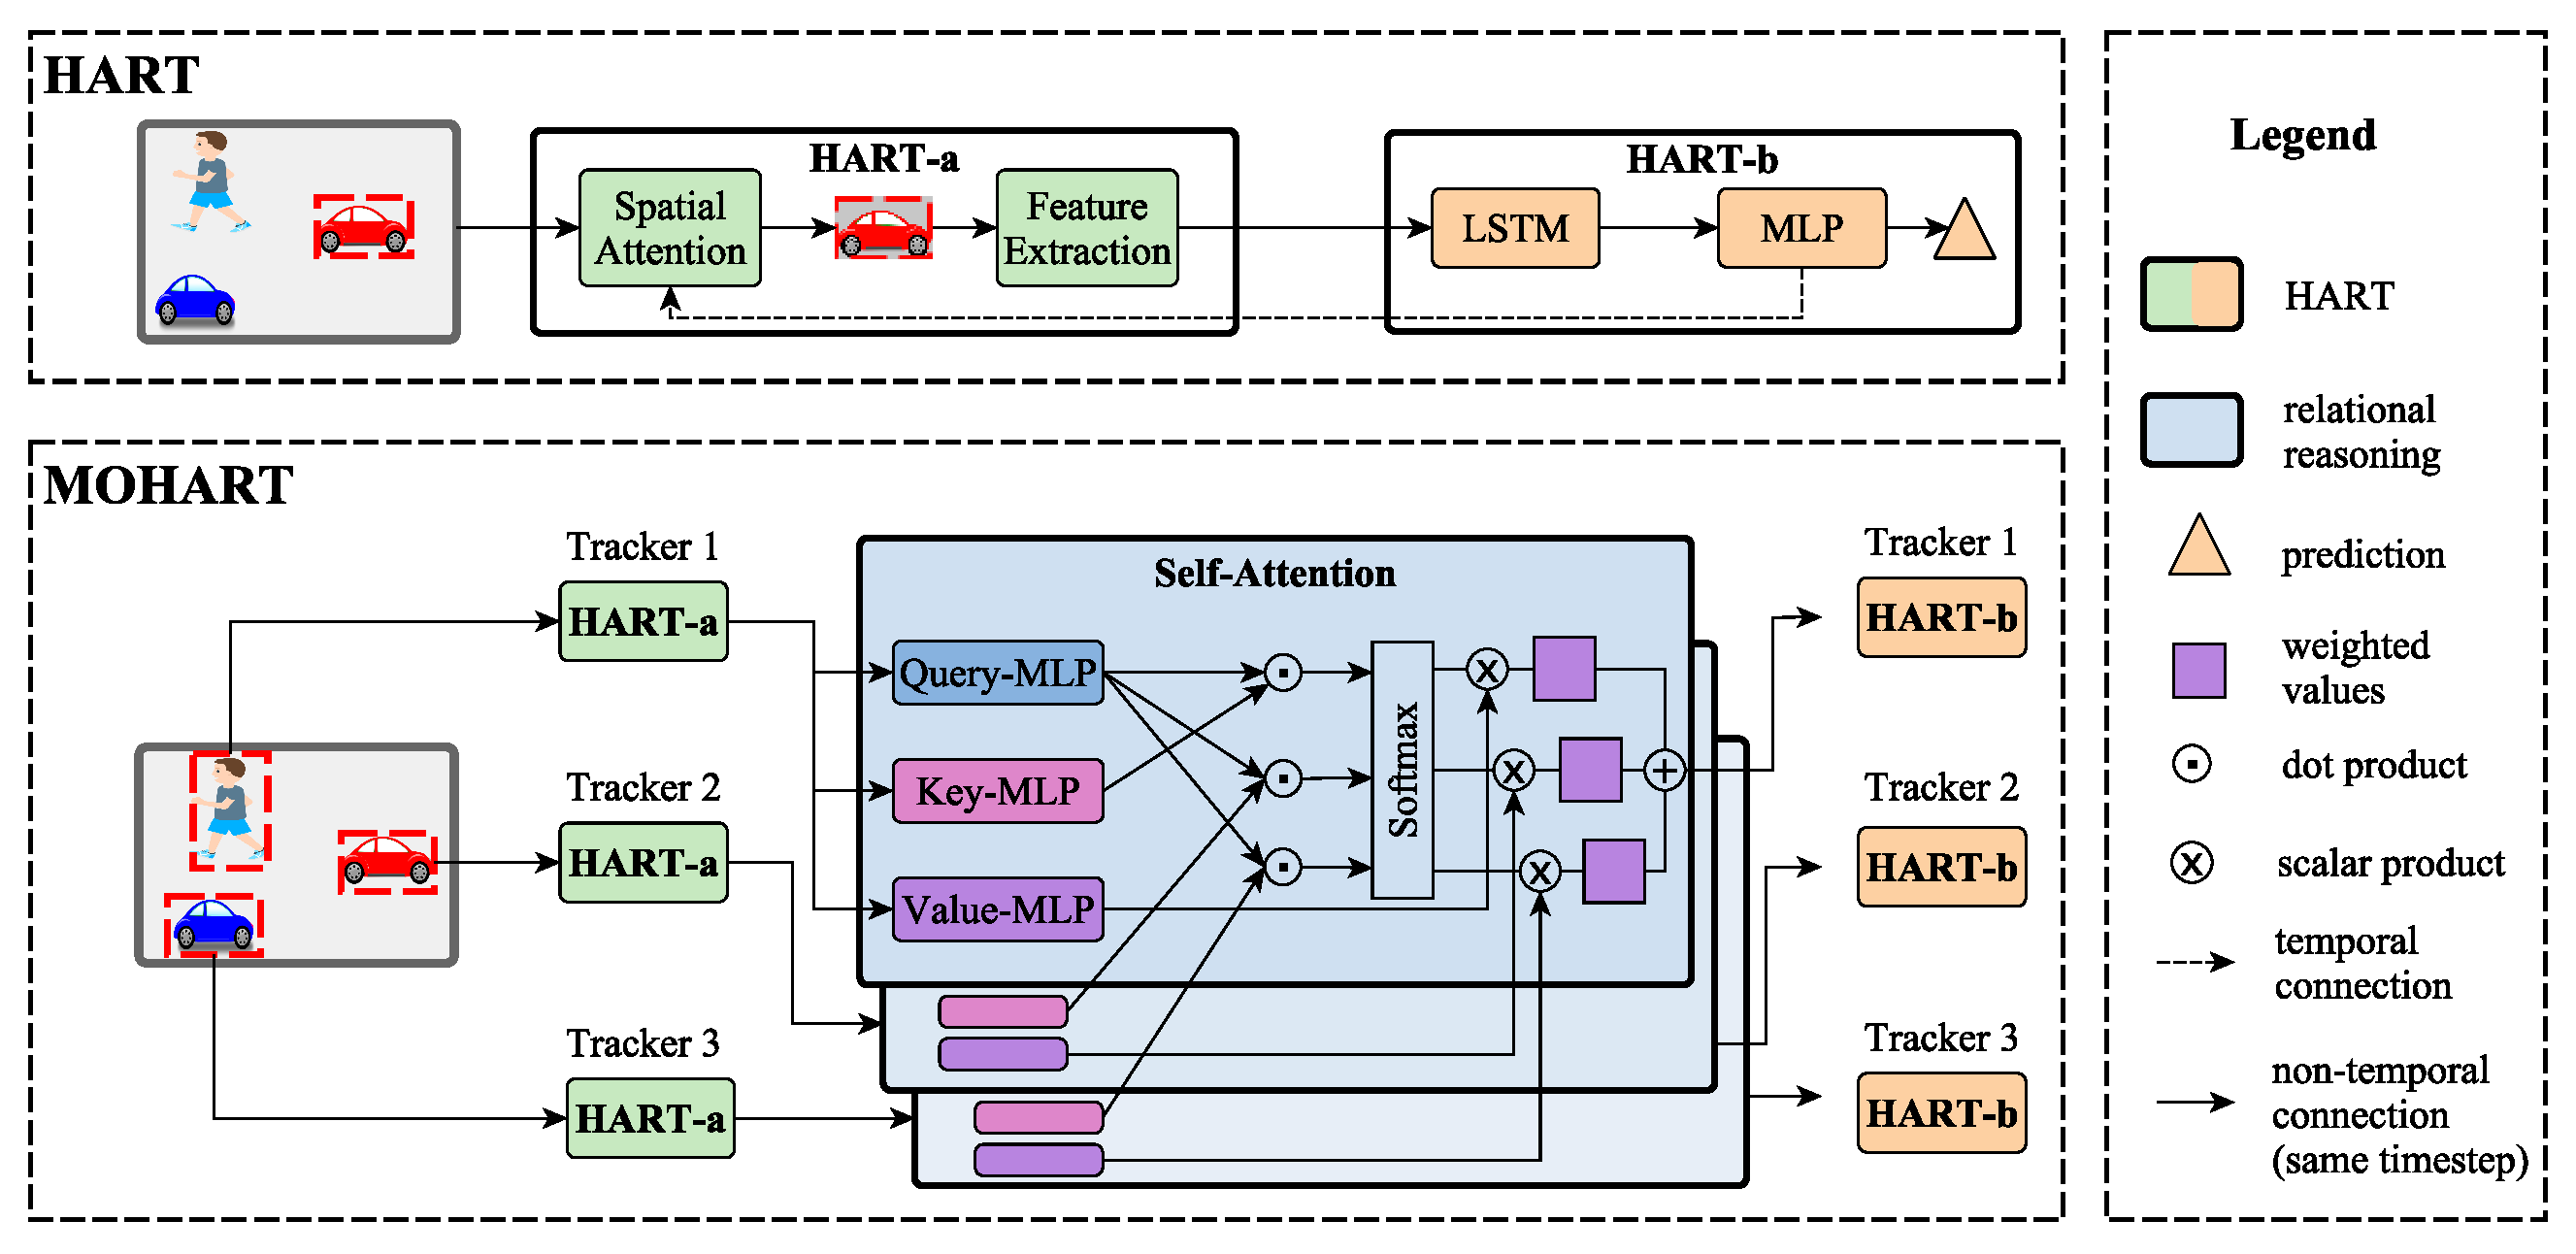
\includegraphics[width=1.0\textwidth]{Figures/system_large.pdf}
	\vspace{-5mm}
	\caption{Single-object tracking with \gls{HART} (top) and our extension to multi-object tracking (\gls{MOHART}, bottom). 
	We track multiple objects in a scene by applying multiple \gls{HART} trackers in parallel. 
	The trackers can exchange information about their respective objects using query-key-value attention.
	To do so, \gls{HART} is split into \gls{HART}-a and \gls{HART}-b (see top row) and we apply the self-attention mechanism in-between the parts.
		\vspace{-2mm}}
	\label{fig:system_large}
\end{figure}

We start by describing the \glsreset{HART}\gls{HART} algorithm \cite{Kosiorek17}, and then follow with an extension of \gls{HART} to tracking multiple objects, where multiple instances of \gls{HART} communicate with each other using multi-headed attention to facilitate relational reasoning. We also explain how this method can be extended to trajectory prediction instead of just tracking. 

\vspace{-.5em}
\paragraph{Hierarchical Attentive Recurrent Tracking (\textsc{hart})}
\textsc{Hart} is an attention-based recurrent algorithm, which can efficiently track single objects in a video.
It uses a spatial attention mechanism to extract a \textit{glimpse} $\bg_t$, which corresponds to a small crop of the image $\bxt$ at time-step $t$, containing the object of interest.
This allows it to dispense with the processing of the whole image and can significantly decrease the amount of computation required.
\Gls{HART} uses a \gls{CNN} to convert the glimpse $\bg_t$ into features $\mathbf{f}_t$, which then update the hidden state $\mathbf{h}_t$ of a \gls{LSTM} core.
The hidden state is used to estimate the current bounding-box $\mathbf{b}_t$, spatial attention parameters for the next time-step $\ba_{t+1}$, as well as object appearance.
Importantly, the recurrent core can learn to predict complicated motion conditioned on the past history of the tracked object, which leads to relatively small attention glimpses---contrary to \gls{CNN}-based approaches \citep{Held2016goturn,Valmadre2017corr}, \gls{HART} does not need to analyse large regions-of-interest to search for tracked objects.
In the original paper, \textsc{hart} processes the glimpse with an additional ventral and dorsal stream on top of the feature extractor. Early experiments have shown that this does not improve performance on the MOTChallenge dataset, presumably due to the oftentimes small objects and overall small amount of training data. 
\Cref{fig:system_large} illustrates \gls{HART}, further details are provided in \Cref{sec:architecture_details}.

	The algorithm is initialised with a bounding-box\footnote{We can use either a ground-truth bounding-box or one provided by an external detector; the only requirement is that it contains the object of interest.} $\mathbf{b}_1$ for the first time-step, and operates on a sequence of raw images $\bx_{1:T}$.
	For time-steps $t\geq2$, it recursively outputs bounding-box estimates for the current time-step and predicted attention parameters for the next time-step. The performance of both algorithms is measured as intersection-over-union (IoU) averaged over all time steps in which an object is present, excluding the first time step.

Although \gls{HART} can track arbitrary objects, it is limited to tracking one object at a time.
While it can  be deployed on several objects in parallel, different \gls{HART} instances have no means of communication.
This results in performance loss, as it is more difficult to identify 
occlusions, ego-motion and object interactions.
Below, we propose an extension of \gls{HART} which remedies these shortcomings.

\vspace{-.5em}
\paragraph{Multi-Object Hierarchical Attentive Recurrent Tracking (\textsc{mohart})}
Multi-object support in \gls{HART} requires the following modifications.
Firstly, in order to handle a dynamically changing number of objects, we apply \gls{HART} to multiple objects in parallel, where all parameters between \gls{HART} instances are shared. 
We refer to each \gls{HART} instance as a \textit{tracker}.
Secondly, we introduce a presence variable $p_{t,m}$ for object $m$.
It is used to mark whether an object should interact with other objects, as well as to mask the loss function (described in \cite{Kosiorek17}) for the given object when it is not present.
In this setup, parallel trackers cannot exchange information and are conceptually still single-object trackers, which we use as a baseline, referred to as \gls{HART} (despite it being an extension of the original algorithm).
Finally, to facilitate communication between trackers, we augment \gls{HART} with an additional step between feature extraction and the \gls{LSTM}.

Let $\mathbf{f}_{t, m}$ be the feature vector extracted from the glimpse corresponding to the m$^\mathrm{th}$ object, and let $\mathbf{f}_{t, 1:M}$ be the set of such features extracted from all glimpses.
Since different objects can interact with each other, it is necessary to use a method that can inform each object about the effects of their interactions with other objects.
Moreover, since features extracted from different objects comprise a set, this method should be permutation-equivariant,\ie the results should not depend on the order in which object features are processed.
Therefore, we use the multi-head self-attention block (\textsc{sab}, \citet{Lee2019settransformer}), which is able to account for higher-order interactions between set elements when computing their representations, thereby allowing rich information exchange, and it can do so in a permutation-equivariant manner.
Intuitively, in our case, \textsc{sab} allows any of the trackers to query other trackers about attributes of their respective objects,\eg distance between objects, their direction of movement, or their relation to the robot.
This is implemented as follows,
\begin{align}
Q &= W_q \mathbf{f}_{1:M} + b_q\,, \qquad K = W_k \mathbf{f}_{1:M} + b_k\,, \qquad V = W_v \mathbf{f}_{1:M} + b_v \label{eq:projection}\,,\\
&\hspace{1.5em} O_i = \operatorname{softmax}\left( Q_i K_i^T \right) V_i\,, \qquad i=1,\dots,H\,, \label{eq:att}\\
&\hspace{7em} o_{1:M} = O = \operatorname{concat}(O_i,\dots,O_H)\,, \label{eq:multihead}
\end{align}
where $o_m$ is the output of the relational reasoning module for object $m$. Time-step subscripts are dropped to decrease clutter.
In \Cref{eq:projection}, each of the extracted features $\mathbf{f}_{t,m}$ is linearly projected into a triplet of key $\mathbf{k}_{t,m}$, query $\mathbf{q}_{t,m}$ and value $\mathbf{v}_{t,m}$ vectors. Together, they comprise $K, Q$ and $V$ matrices with $M$ rows and $d_q, d_k, d_k$ columns, respectively.
$K, Q$ and $V$ are then split up into multiple heads $H \in \mathbb{N}_+$, which allows to query different attributes by comparing and aggregating different projection of features.
Multiplying $Q_iK_i^T$ in \Cref{eq:att} allows to compare every query vector $\mathbf{q}_{t,m,i}$ to all key vectors $\mathbf{k}_{t,1:M,i}$, where the value of the corresponding dot-products represents the degree of similarity.
Similarities are then normalised via a $\operatorname{softmax}$ operation and used to aggregate values $V$.
Finally, outputs of different attention heads are concatenated in \Cref{eq:multihead}.
\textsc{Sab} produces $M$ output vectors, one for each input, which are then concatenated with corresponding inputs and fed into separate \gls{LSTM}s for further processing, as in \gls{HART}---see \Cref{fig:system_large}.

\Gls{MOHART} is trained fully end-to-end, contrary to other tracking approaches \cite{Zhang2008,Milan2014,bae2017confidence,keuper2018motion}.
It maintains a hidden state, which can contain information about the object's motion. One benefit is that in order to predict future trajectories, one can simply feed black frames into the model. Our experiments show that the model learns to fall back on the motion model captured by the \gls{LSTM} in this case. 


